\title{K-Means Parallelization \\
	Final Project Design Specification}
\author{Brian Dunlay\\
	EE590A - Winter 2017
}
\date{\today}

\documentclass[11pt]{article}
\usepackage{amsfonts}
\usepackage{mathtools}
\newcommand{\BigO}[1]{\ensuremath{\operatorname{O}\bigl(#1\bigr)}}

\begin{document}
\maketitle

\section*{Introduction}
I spent much of my time preparing for this design spec by implementing the algorithm in
C++ to get a sequential reference. What I found was that the algorithm itself is actually
fairly simple, and it naturally benefits from the parallelism provided by GPUs due to
the inherent data independence in evaluating mean euclidean distance for each point.

What I found difficult was the book-keeping of centroid assignment. Either each pixel
in global memory must be annotated with its centroid and processed sequentially, or independent
vectors must be formed (with synchronization) that can be re-submitted to the GPU for processing.

I have outlined a half-GPU half-CPU implementation, but I am going to experiment
in the development of my parallel algorithm with synchronizing writes to shared memory vectors.

\section{K-Means Equations}

K-means is a clustering algorithm. Given an integer $k$ and a set of $n$ data points $X \subset \mathbb{R}^d$ we aim to choose $k$ centers $C$ so as to minimize the following function \cite{arthur}:
\newline

\begin{math}
\phi = \displaystyle\sum_{x \in X} min_{c \in C }\| x - c \|^2
\end{math}

\subsection{Iterative Algorithm}
The algorithm can be implemented in three steps:

\begin{enumerate}
\item Arbitrarily choose an initial k centers $C = {c_1, c_2, \cdots, c_k}$
\item For each $i \in {1, \cdots, k}$, set the cluster $C_i$ to be the set of points in $X$ that are closer to $c_i$ than they are to $c_j$ for all $j \neq i$
\item For each $i \in {1, \cdots, k}$, set $c_i$ to be the center of mass of all points in $C_i$: $c_i = \frac{1}{|C_i|}\sum_{x \in C_i}x$
\item Repeat Steps 2 and 3 until $C$ no longer changes
\end{enumerate}

\section{Sequential Reference}

I wrote a sequential reference in C++ in order to achieve a baseline. I found that
it is less computationally intensive to convert the image to the YUV color space and
do a comparison (euclidean distance) between points than it would have been to do
the same in RGB colorspace.

I did not time the colorspace conversions given the fact that it is not relevant to the
immediate problem (K-Means clustering), however the conversion would be easily
parallelizable.

For a visual indication of the result of the k-means clustering, I colorized the clusters
based upon their mean color value along with a constant luma value. This was also omitted
from the timing of the runtime.

\subsection{Sample Image}

\begin{figure}[ht]
    \centering
    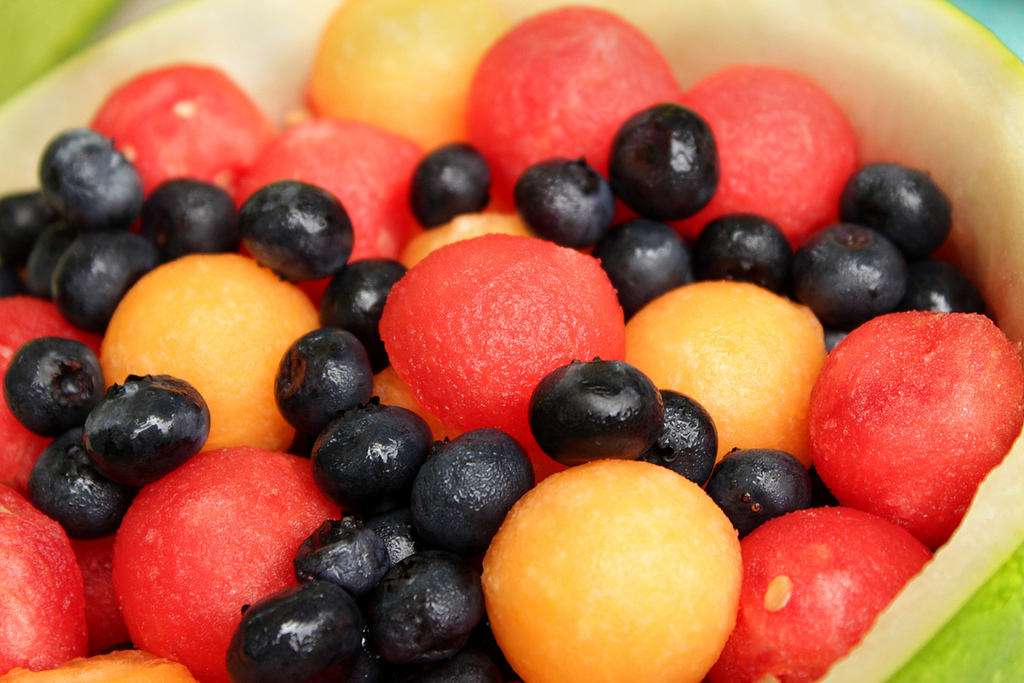
\includegraphics[width=0.6\textwidth]{fruit.png}
    \caption{Image\cite{fruit} before segmentation}
    \label{fig:fruit}
\end{figure}

\begin{figure}[ht]
    \centering
    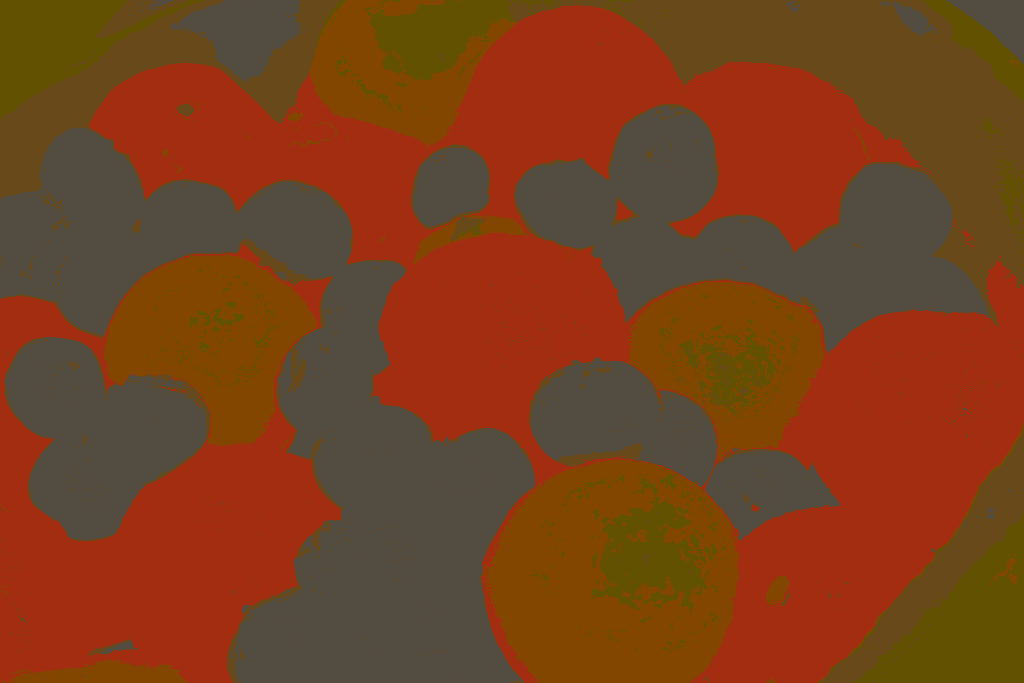
\includegraphics[width=0.6\textwidth]{fruit-segmented.png}
    \caption{Image after segmentation}
    \label{fig:fruit-segmented}
\end{figure}

This image was segmented based on 5 coordinates that were hand-picked as input to the program.
The average runtime over 30 runs for processing this image was 3.026 seconds.

See \emph{results.txt} for individual runtime samples.

\subsection{Code}

See \emph{sequential-kmeans.cpp} for the sequential code reference implementation.

\section{Complexity Analysis}

\subsection{Algorithmic Complexity}

There are two primary stages of this algorithm, and I will analyize each of them individually.
It should be noted that sinces the algorithm is iterative until convergence is reached, there
is a unknown factor in which we will recalculate the following two steps. In most cases it
should be much less than N.

\subsubsection{Clustering}

The first stage is clustering each pixel in the image with an associated group. For
each pixel $x_i$ in the image, we compute the euclidean distance between $x_i$
and each centroid $c_i$ with dimensionality $D$.

$\BigO{NKD}$

Where $N$ is the number of pixels in the image and $K$ is the number of centroids. As
previously mentioned, there is a slight reduction in the algorithmic complexity by
reducing the dimensionality of the colorspace from 3 (RGB) to 2 (U and V of YUV).

$D$ could technically be omitted given that it is a constant that is likely smaller
than $K$ and likely significantly smaller than $N$.

\subsubsection{Mean centroid calculation}

The second stage is to calculate the average value for all pixels in a particular cluster $c_i = \frac{1}{|C_i|}\sum_{x \in C_i}x$. The algorithmic complexity is: $\BigO{ND}$ where we are calculating a summation of $D$ values over $N$ data points.

\subsection{Arithmetic Intensity}

The arithmetic intensity for the clustering step is $K$ iterations of a (1) the difference between two centroids (2) squared and (3) summed over $D$ dimensions, followed by a (4) square root. $\text{FLOPS} = K(3D+1)$.

The data access of the clustering step is $KD+D$ reads (where one byte is read per dimension) and the $1$ write (the cluster id) for a total of $KD+D+1$.

The AI is therefore $\frac{K3D+K}{KD+D+1}$

\section{Parallel Pseudo-Code}

See \emph{parallel-kmeans.cl} for the parallel pseudo-code implementation.

\begin{thebibliography}{9}

\bibitem{arthur}
  David Arthur and Sergei Vassilvitskii,
  \emph{k-means++: The Advantages of Careful Seeding},
  http://ilpubs.stanford.edu:8090/778/1/2006-13.pdf

\bibitem{mipro}
  J. Sirotkovi, H.Dujmi, V. Papi
  \emph{K-Means Image Segmentation on Massively Parallel GPU Architecture}

\bibitem{fruit}
  Didriks,
  \emph{Fruit Salad},
  https://flic.kr/p/a6W1Te

\end{thebibliography}

\end{document}
This is never printed
